\documentclass[a4]{article}

\usepackage[left=3cm,right=3cm,top=2cm,bottom=2cm]{geometry} 

\usepackage[utf8]{inputenc}   % otra alternativa para los caracteres acentuados y la "ñ"
\usepackage[           spanish % para poder usar el español
                      ,es-tabla % para los captions de las tablas
                       ]{babel}   
\decimalpoint %para usar el punto decimal en vez de coma para los números con decimales

\usepackage[T1]{fontenc}
\usepackage{lmodern}

\usepackage{parskip}
\usepackage{xcolor}

\usepackage{caption}

\usepackage{enumerate}% paquete para poder personalizar fácilmente la apariencia de las listas enumerativas

\usepackage{graphicx} % figuras
\usepackage{subfigure} % subfiguras

\definecolor{gris}{RGB}{220,220,220}
	
\usepackage{float} % para controlar la situación de los entornos flotantes

\restylefloat{figure}
\restylefloat{table} 

\newcommand{\HRule}{\rule{\linewidth}{0.5mm}}

\author{David Cabezas Berrido}
\date{\vspace{-5mm}}

\title{\huge Práctica 1: Eficienca \HRule\vspace{-4mm}}

\begin{document}

\maketitle

\tableofcontents

\section{Eficiencia Empírica}

\begin{table}[H]
\begin{minipage}{0.45\linewidth}
\centering
\title{\large Algoritmos con eficiencia $O(n^2)$\vspace{4mm}}
\begin{tabular}{| c c c c |}
\hline
$\textbf{n}$ & \textbf{Burbuja} & \textbf{Inserción} & \textbf{Selección} \\ \hline
  1000  & 0.004416 & 0.001242 & 0.00132932 \\ 
  2000  & 0.009701 & 0.005147 & 0.00472456 \\ 
  3000  & 0.021534 & 0.012807 & 0.010695   \\ 
  4000  & 0.033732 & 0.020767 & 0.018866   \\ 
  5000  & 0.052993 & 0.024215 & 0.029365   \\ 
  6000  & 0.0785   & 0.034137 & 0.042309   \\ 
  7000  & 0.116606 & 0.046124 & 0.057128   \\ 
  8000  & 0.157316 & 0.059695 & 0.074368   \\ 
  9000  & 0.198552 & 0.074662 & 0.093737   \\ 
  10000 & 0.244325 & 0.092759 & 0.115629   \\ 
  11000 & 0.297715 & 0.11217  & 0.140806   \\ 
  12000 & 0.355768 & 0.13501  & 0.166908   \\ 
  13000 & 0.421353 & 0.157762 & 0.195358   \\
  14000 & 0.490008 & 0.182619 & 0.226432   \\
  15000 & 0.565647 & 0.208906 & 0.260561   \\
  16000 & 0.648838 & 0.239027 & 0.294718   \\
  17000 & 0.734952 & 0.266649 & 0.334074   \\
  18000 & 0.825036 & 0.301845 & 0.373655   \\
  19000 & 0.925171 & 0.334605 & 0.416012   \\
  20000 & 1.02862  & 0.368961 & 0.461119   \\
  21000 & 1.13798  & 0.407094 & 0.508379   \\
  22000 & 1.2548   & 0.448405 & 0.558152   \\
  23000 & 1.37147  & 0.491561 & 0.608983   \\
  24000 & 1.53636  & 0.537183 & 0.662848   \\
  25000 & 1.67428  & 0.586868 & 0.719359   \\ \hline
\end{tabular}
\end{minipage}

\hfill

\begin{minipage}{0.45\linewidth}
\centering
\title{\large Algoritmos con eficiencia $O(n\log n)$\vspace{4mm}}
\begin{tabular}{| c c c c |}
\hline
$\textbf{n}$ & \textbf{Mergesort} & \textbf{Quicksort} & \textbf{Heapsort} \\ \hline
  1000  & 0.000111503 & 0.000349 & 0.000452 \\ 
  2000  & 0.000235082 & 0.000921 & 0.001106 \\ 
  3000  & 0.000433307 & 0.000349 & 0.001416 \\ 
  4000  & 0.000507335 & 0.000482 & 0.000682 \\ 
  5000  & 0.000711784 & 0.000606 & 0.000806 \\ 
  6000  & 0.000933769 & 0.000764 & 0.000984 \\ 
  7000  & 0.000906519 & 0.00101  & 0.001154 \\ 
  8000  & 0.00109287  & 0.001136 & 0.001349 \\ 
  9000  & 0.0012998   & 0.001303 & 0.001527 \\ 
  10000 & 0.00151355  & 0.001499 & 0.001716 \\ 
  11000 & 0.001805    & 0.001428 & 0.002097 \\ 
  12000 & 0.002079    & 0.001595 & 0.002104 \\ 
  13000 & 0.001935    & 0.001735 & 0.002302 \\
  14000 & 0.001973    & 0.001877 & 0.002499 \\
  15000 & 0.002167    & 0.002125 & 0.002801 \\
  16000 & 0.002389    & 0.002158 & 0.002912 \\
  17000 & 0.002663    & 0.002309 & 0.003118 \\
  18000 & 0.002867    & 0.002161 & 0.003316 \\
  19000 & 0.003284    & 0.002223 & 0.00357  \\
  20000 & 0.003441    & 0.002341 & 0.003735 \\
  21000 & 0.003775    & 0.002306 & 0.003925 \\
  22000 & 0.004023    & 0.002397 & 0.003771 \\
  23000 & 0.004289    & 0.002619 & 0.003569 \\
  24000 & 0.004311    & 0.002889 & 0.003566 \\
  25000 & 0.004956    & 0.002906 & 0.003972 \\ \hline
\end{tabular}
\end{minipage}
\end{table}

\begin{table}[H]
\begin{minipage}{0.4\textwidth}
\centering
\title{\large Algoritmos con eficiencia $O(n^3)$ \\ \vspace{4mm}}
\begin{tabular}{| c c |}
\hline
$\textbf{n}$ & \textbf{Floyd} \\ \hline
  100  & 0.007701 \\ 
  200  & 0.046747 \\ 
  300  & 0.132648 \\ 
  400  & 0.308783 \\ 
  500  & 0.602721 \\ 
  600  & 1.03593  \\ 
  700  & 1.64485  \\ 
  800  & 2.44615  \\ 
  900  & 3.609    \\ 
  1000 & 4.7692   \\ 
  1100 & 6.35587  \\ 
  1200 & 8.29301  \\ 
  1300 & 10.4978  \\
  1400 & 13.1335  \\
  1500 & 16.3889  \\
  1600 & 19.623   \\
  1700 & 23.5916  \\
  1800 & 28.0699  \\
  1900 & 32.8918  \\
  2000 & 38.2142  \\
  2100 & 44.9125  \\
  2200 & 50.9494  \\
  2300 & 58.9452  \\
  2400 & 66.1602  \\
  2500 & 74.5625  \\ \hline
\end{tabular}
\end{minipage}

\hfill

\begin{minipage}{0.4\textwidth}
\centering
\title{\large Algoritmos con eficiencia $O(2^n)$ \\ \vspace{4mm}}
\begin{tabular}{| c c |}
\hline
$\textbf{n}$ & \textbf{Hanoi} \\ \hline
  10 &	2.8e-05  \\
  11 &	5.3e-05  \\
  12 &	0.000101 \\
  13 &	5.4e-05  \\
  14 &	0.000108 \\
  15 &	0.000221 \\
  16 &	0.000457 \\
  17 & 	0.000909 \\
  18 &	0.001828 \\
  19 &	0.003638 \\
  20 &	0.007117 \\
  21 &	0.012896 \\
  22 &	0.025344 \\
  23 &	0.04889  \\
  24 &	0.090453 \\
  25 &	0.181502 \\
  26 &	0.361282 \\
  27 &	0.739665 \\
  28 &	1.43885  \\
  29 &	2.87849  \\
  30 &	5.8083   \\
  31 &	11.5332  \\
  32 &	23.0484  \\
  33 &	46.2319  \\
  34 &	93.0055  \\
  35 &	184.521  \\ \hline
\end{tabular}
\end{minipage}
\end{table}

\section{Gráficos}

\begin{figure}[H]
  \centering
  \subfigure[Algoritmos con eficiencia $O(n^2)$]{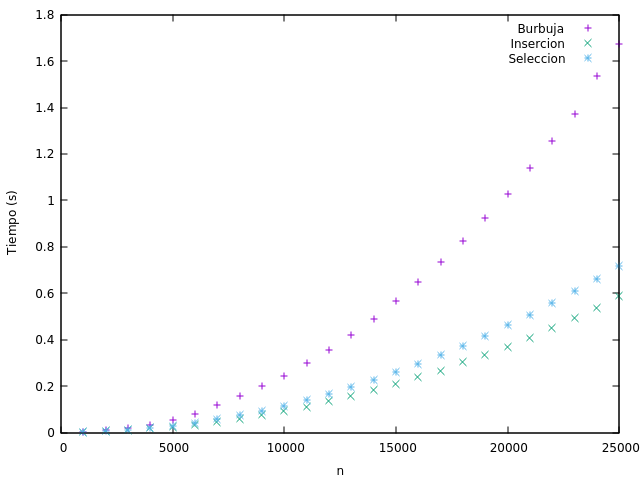
\includegraphics[width=70mm]{graficos/on2}}
  \subfigure[Algoritmos con eficiencia $O(n\log n)$]{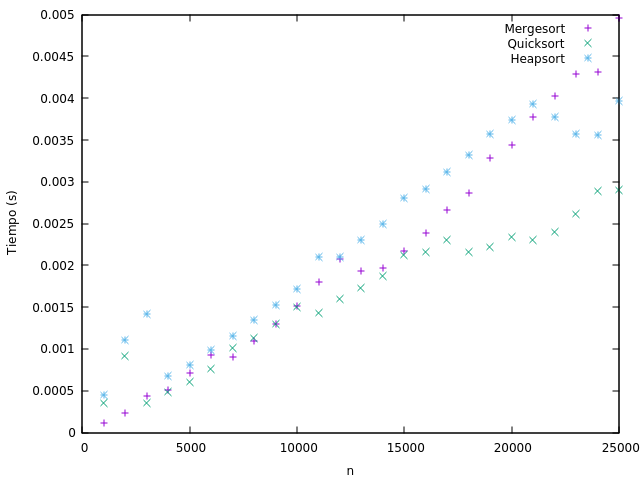
\includegraphics[width=70mm]{graficos/onlogn}}
  \subfigure[Algoritmos con eficiencia $O(n^3)$]{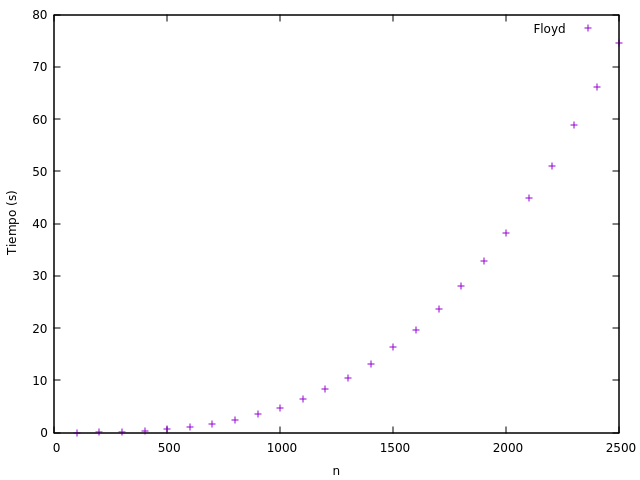
\includegraphics[width=70mm]{graficos/on3}}
  \subfigure[Algoritmos con eficiencia $O(2^n)$]{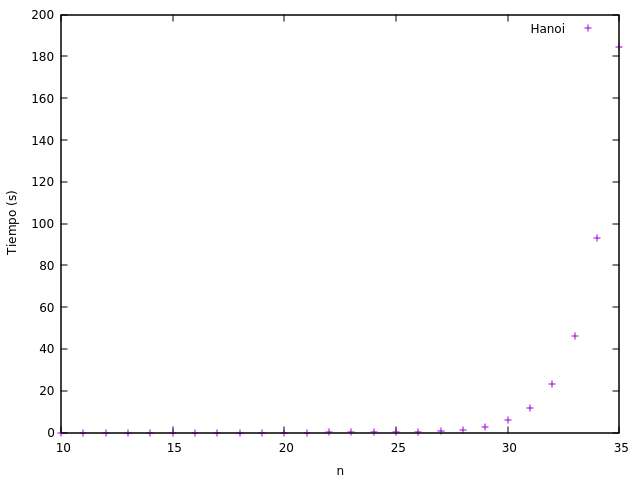
\includegraphics[width=70mm]{graficos/o2n}}
  \subfigure[Algoritmos de ordenación]{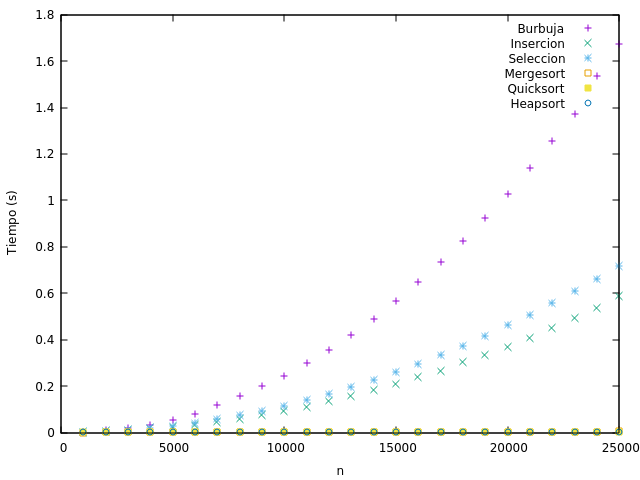
\includegraphics[width=90mm]{graficos/sort}}
\end{figure}

\section{Eficiencia Híbrida}

\subsection{Algoritmos con eficiencia $O(n^2)$}

\begin{flushleft}
  Usando la orden fit, he ajustado los resultados de estos algoritmos
  con una función de la forma \[\hspace{-30mm}f(x)=a_0x^2+a_1x+a_2\] A
  continuación expongo los distintos coeficientes que he obtenido en
  el ajuste de los tiempos de cada algoritmo, junto con una
  represención de la función y los resultados.
\end{flushleft}

\subsubsection{Burbuja}

\begin{verbatim}
Final set of parameters            Asymptotic Standard Error
=======================            ==========================
a0              = 2.87309e-09      +/- 3.994e-11    (1.39%)
a1              = -6.33841e-06     +/- 1.07e-06     (16.88%)
a2              = 0.014873         +/- 0.006036     (40.59%)
\end{verbatim}

\begin{figure}[H]
  \centering
  \subfigure{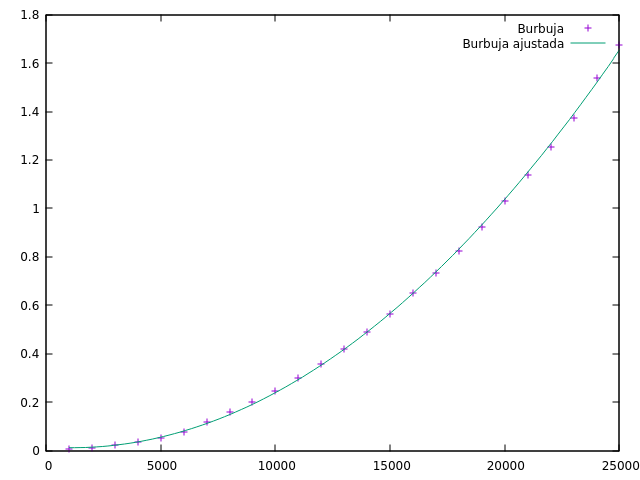
\includegraphics[width=70mm]{graficos/burbuja_ajust}}
\end{figure}

\subsubsection{Inserción}

\begin{verbatim}
Final set of parameters            Asymptotic Standard Error
=======================            ==========================
a0              = 9.49226e-10      +/- 8.518e-12    (0.8974%)
a1              = -5.93381e-07     +/- 2.282e-07    (38.45%)
a2              = 0.0039437        +/- 0.001287     (32.64%)
\end{verbatim}

\begin{figure}[H]
  \centering
  \subfigure{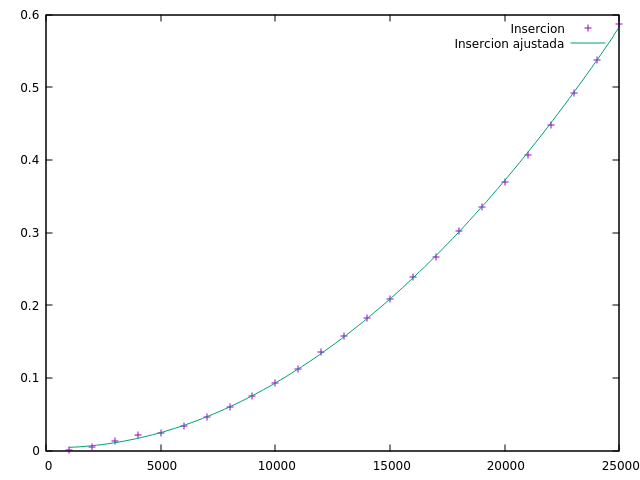
\includegraphics[width=70mm]{graficos/insercion_ajust}}
\end{figure}

\subsubsection{Selección}
\begin{verbatim}
Final set of parameters            Asymptotic Standard Error
=======================            ==========================
a0              = 1.14435e-09      +/- 1.562e-12    (0.1365%)
a1              = 1.72508e-07      +/- 4.185e-08    (24.26%)
a2              = -0.000123672     +/- 0.0002361    (190.9%)
\end{verbatim}

\begin{figure}[H]
  \centering
  \subfigure{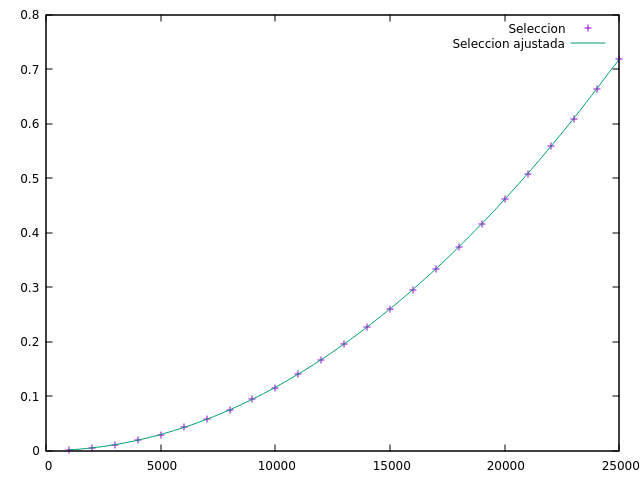
\includegraphics[width=70mm]{graficos/seleccion_ajust}}
\end{figure}

\subsection{Algoritmos con eficiencia $O(n\log n)$}

\begin{flushleft}
  Usando la orden fit, he ajustado los resultados de estos algoritmos
  con una función de la forma \[\hspace{-30mm}f(x)=an\log(bx+c)+d\] A
  continuación expongo los distintos coeficientes que he obtenido en
  el ajuste de los tiempos de cada algoritmo, junto con una
  represención de la función y los resultados.
\end{flushleft}

\subsubsection{Mergesort}

\begin{verbatim}
Final set of parameters            Asymptotic Standard Error
=======================            ==========================
a               = 6.95655e-08      +/- 1.431e-08    (20.57%)
b               = 0.000491397      +/- 0.0002775    (56.47%)
c               = 7.18312e-07      +/- 9.373e+04    (1.305e+13%)
d               = 0.000312996      +/- 13.27        (4.239e+06%)
\end{verbatim}

\begin{figure}[H]
  \centering
  \subfigure{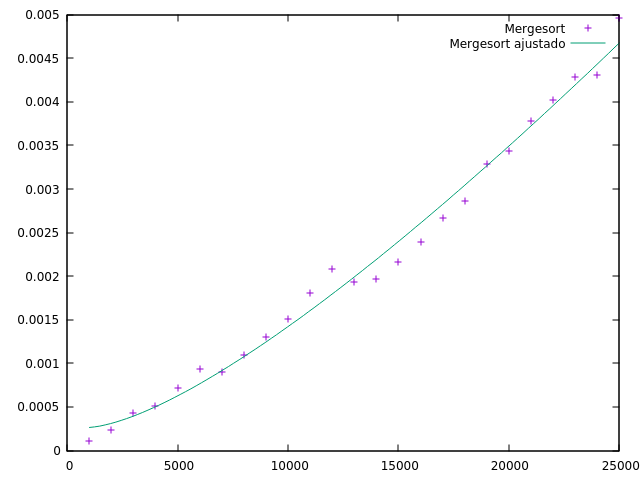
\includegraphics[width=70mm]{graficos/mergesort_ajust}}
\end{figure}

\subsubsection{Quicksort}

\begin{verbatim}
Final set of parameters            Asymptotic Standard Error
=======================            ==========================
a               = 1.07312e-08      +/- 1.716e-08    (159.9%)
b               = 0.542892         +/- 8.438        (1554%)
c               = 7.18316e-07      +/- 2.12e+05     (2.951e+13%)
d               = 0.000390981      +/- 0.004212     (1077%)
\end{verbatim}

\begin{figure}[H]
  \centering
  \subfigure{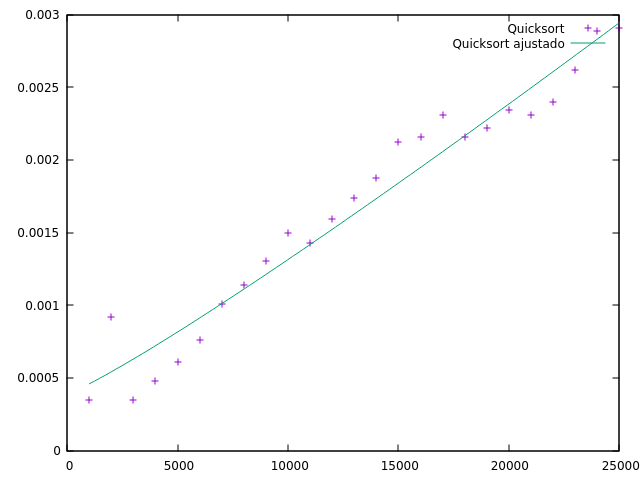
\includegraphics[width=70mm]{graficos/quicksort_ajust}}
\end{figure}

\subsubsection{Heapsort}

\begin{verbatim}
Final set of parameters            Asymptotic Standard Error
=======================            ==========================
a               = 2.02343e-08      +/- 2.677e-08    (132.3%)
b               = -0.0611422       +/- 0.6122       (1001%)
c               = 2.74491e-06      +/- 7.44e+05     (2.711e+13%)
d               = 0.000535336      +/- 0.2463       (4.6e+04%)
\end{verbatim}

\begin{figure}[H]
  \centering
  \subfigure{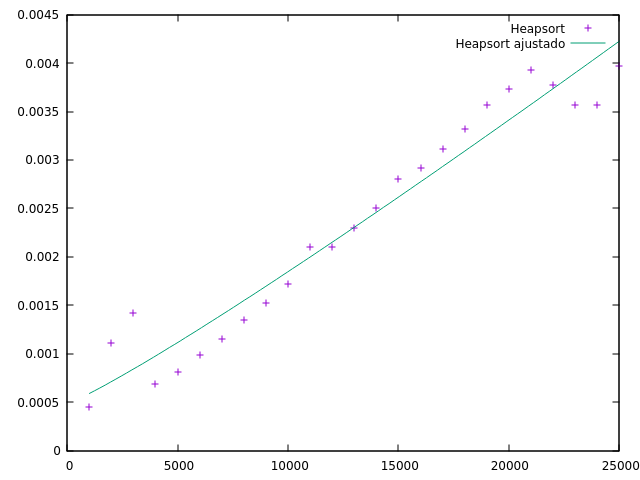
\includegraphics[width=70mm]{graficos/heapsort_ajust}}
\end{figure}

\subsection{Algoritmos con eficiencia $O(n^3)$: Floyd}

Usando la orden fit, he ajustado los resultados de estos algoritmos
con una función de la
forma \[\hspace{-30mm}f(x)=a_0x^3+a_1x^2+a_2x+a_3\] A continuación
expongo los distintos coeficientes que he obtenido en el ajuste de los
tiempos de cada algoritmo, junto con una represención de la función y
los resultados.

\begin{verbatim}
Final set of parameters            Asymptotic Standard Error
=======================            ==========================
a0              = 4.6365e-09       +/- 1.322e-10    (2.851%)
a1              = 5.80584e-07      +/- 5.222e-07    (89.94%)
a2              = -0.00053539      +/- 0.0005904    (110.3%)
a3              = 0.111407         +/- 0.1808       (162.3%)
\end{verbatim}

\begin{figure}[H]
  \centering
  \subfigure{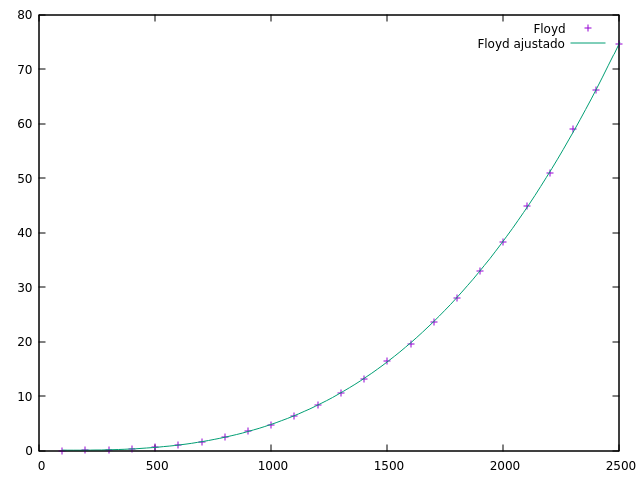
\includegraphics[width=70mm]{graficos/floyd_ajust}}
\end{figure}

\subsection{Algoritmos con eficiencia $O(2^n)$: Hanoi}

Usando la orden fit, he ajustado los resultados de estos algoritmos
con una función de la
forma \[\hspace{-30mm}f(x)=a2^x+b\] A continuación
expongo los distintos coeficientes que he obtenido en el ajuste de los
tiempos de cada algoritmo, junto con una represención de la función y
los resultados.

\begin{verbatim}
Final set of parameters            Asymptotic Standard Error
=======================            ==========================
a               = 5.33528e-09      +/- 2.615e-11    (0.49%)
b               = 1                +/- 0.2034       (20.34%)
\end{verbatim}

\begin{figure}[H]
  \centering
  \subfigure{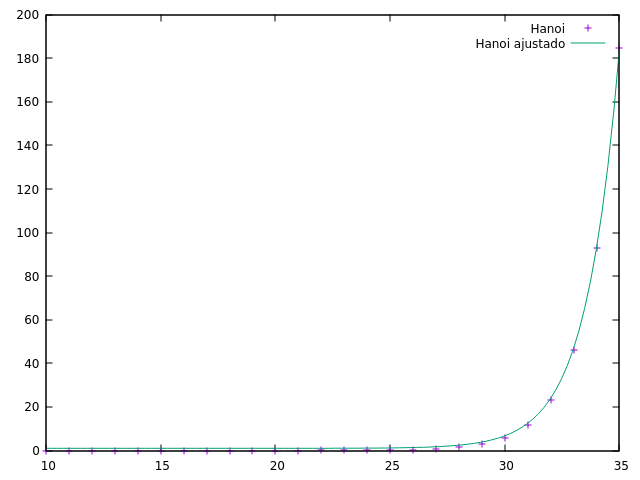
\includegraphics[width=70mm]{graficos/hanoi_ajust}}
\end{figure}

\end{document}